\documentclass[%
	paper=a4,%
	twoside=true,%
	draft=false,%
	abstract=false]{scrartcl}

\usepackage[utf8]{inputenc}
\usepackage[english]{babel}
\usepackage{microtype}
\usepackage{graphicx}
\usepackage[load-configurations=binary]{siunitx}
	\DeclareSIUnit\Molar{\textsc{m}}
\usepackage{svn-multi}
\usepackage{subfig}
\usepackage{booktabs}
\usepackage{fancyhdr}
\usepackage{tikz}
\usepackage{pgfplots}
\usepackage[numbers,square,sort&compress]{natbib}
\usepackage{scrtime}
\usepackage[version=3]{mhchem}
\usepackage{setspace}
	%\doublespacing
	%\onehalfspacing
\usepackage{lineno}
	\linenumbers\modulolinenumbers[2]
\usepackage{lastpage}	
\usepackage{xspace}
\usepackage[colorinlistoftodos,shadow]{todonotes}
\usepackage[autostyle]{csquotes}
\usepackage[backref]{hyperref}
 
% Subversion Information
\svnidlong
{$HeadURL$}
{$LastChangedDate$}
{$LastChangedRevision$}
{$LastChangedBy$}
\svnid{$Id$} 
 
\pagestyle{fancy}
\fancyfoot{}
\fancyfoot[OR]{\tiny Typeset on \today\ at \thistime\ from \href{\svnkw{HeadURL}}{Revision \svnkw{LastChangedRevision}}, committed on \svnkw{LastChangedDate} | Page \thepage\ of \pageref{LastPage}}
\fancyfoot[EL]{\tiny Page \thepage\ of \pageref{LastPage} | Typeset on \today\ at \thistime\ from \href{\svnkw{HeadURL}}{Revision \svnkw{LastChangedRevision}}, committed on \svnkw{LastChangedDate}}
 
\newcommand{\imsize}{\linewidth}

\newcommand{\footremember}[2]{\footnote{#2}\newcounter{#1}\setcounter{#1}{\value{footnote}}}
\newcommand{\footrecall}[1]{\footnotemark[\value{#1}]}

\newcommand{\superscript}[1]{\ensuremath{^{\textrm{#1}}}}
\newcommand{\subscript}[1]{\ensuremath{_{\textrm{#1}}}}

\newcommand{\ie}{i.\,e.\xspace}
\newcommand{\Ie}{I.\,e.\xspace}
\newcommand{\eg}{e.\,g.\xspace}
\newcommand{\Eg}{E.\,g.\xspace}
\newcommand{\twod}{2\textsc{d}\xspace}
\newcommand{\threed}{3\textsc{d}\xspace}

\newcommand{\todomarco}[2][]{\todo[color=cyan!62!white,, #1]{Marco: #2}}
\newcommand{\todojcs}[2][]{\todo[color=magenta!62!white, #1]{Johannes: #2}}
\newcommand{\todome}[2][]{\todo[color=yellow!62!white, #1]{David: #2}}

\newcommand{\subfigureautorefname}{\figureautorefname} % make \autoref work with \subfloat
 
\title{Acinar growth over lung development}
\subtitle{Revision \svnkw{LastChangedRevision} | Typeset on \today\ at \thistime}

\author{%
	David Haberthür\footremember{ana}{Institute of Anatomy, University of Bern, Switzerland}%
	\and Marco Stampanoni\footremember{psi}{Swiss Light Source, Paul Scherrer Institut, Villigen, Switzerland}\footremember{eth}{Institute for Biomedical Engineering, Swiss Federal Institute of Technology and University of Zürich, Switzerland}%
	\and Johannes C. Schittny\footrecall{ana}%
	}
\date{}

\begin{document}
\maketitle

\begin{abstract}
Here be the Abstract\ldots
\end{abstract}

\listoftodos

\section{Introduction}\label{sec:Introduction}
Due a restricted availability of high resolution three-dimensional imaging methods the knowledge about the development of the functional unit of the lung is limited. These functional units of the lung parenchyma are the so called pulmonary acini, which correspond to the gas-exchange volume in the lung which is ventilated by one purely conducting airway~\cite{Rodriguez1987}.\todo{Size and more info?} Using synchrotron radiation based tomographic microscopy \cite{Haberthuer2010a} we developed a method to evaluate the volume of single acini throughout postnatal lung development\todo{Why did we want to do that? Do we need to list/explain existing prior models?}. In pre-experiments assessing the lung structure using three-dimensional visualizations of synchrotron radiation based tomographic microscopy datasets we have seen that the functional lung units---the so-called acini---seen to grow to a larger extent than expected from \emph{simple} lung development.

The lung structure can be assessed using stereology~\cite{Hsia2010}, as shown by \citet{Tschanz2002}. Such an analysis is generally based on serial sections of the sample, thus the extracted information is a two-dimensional description \blockquote[\cite{Tschanz2002}]{of the parenchymal air space geometry and, due to geometric laws, it is not allowed to extrapolate these \twod statements directly to \threed structures}. With stereological methods it is fairly easy to extract global volume information\todojcs{From a region, from a ROI?}, but it not easily possible to extract such information from a functional unit of any organ, since it cannot easily be judged which detail on the microscopy slide belong to which functional unit in the three-dimensional compound.

\section{Materials \& Methods}\label{sec:MM}
\subsection{Rat lung samples}
We used rat lung samples, prepared according to \cite{Tschanz2002,Luyet2002}. Briefly, lungs of Sprague-Dawley rats were instilled with \SI{2.5}{\percent} glutaraldehyde (\cf{CH2(CH2CHO)2}) in \SI{0.03}{\Molar} potassium-phosphate buffer (pH 7.4) at a constant pressure of \SI{20}{\centi\meter} water column via tracheotomy. This pressure was maintained during the fixation (in the same fixative at \SI{4}{\celsius} for at least \SI{24}{\hour}) in order to prevent a recoiling and to preserve a mid-respiratory\todojcs{Is mid-respiratory true, or is this full volume?} state of the lung.

To prepare the samples for tomographic imaging, they were postfixed with \SI{1}{\percent} osmium tetroxide (\cf{OsO4}) and stained with \SI{4}{\percent} uranyl nitrate (\cf{UO2(NO3)2}) to increase the x-ray absorption contrast, dehydrated in a graded series of ethanol and embedded in paraffin using Histoclear (Merck KGaA, Darmstadt, Germany) as an intermedium. Subsequently, the lung samples were mounted onto standard scanning electron microscopy sample holders (PLANO GmbH, Wetzlar, Germany) using paraffin~\cite{Tsuda2008}. After this processing, the samples can be regarded as inert and can be kept as long as desired prior to tomographic scanning.

The handling of animals before and during the experiments, as well as the experiments themselves, were approved and supervised by the Swiss Agency for the Environment, Forests and Landscape and the Veterinary Service of the Canton of Bern, Switzerland.

\subsection{Tomographic data acquisition}\label{sec:tomcat}
All tomographic experiments for this publication were performed at the \href{http://www.psi.ch/sls/tomcat/}{TOMCAT beamline} at the \href{http://www.psi.ch/sls/}{Swiss Light Source}, \href{http://www.psi.ch/}{Paul Scherrer Institut}, Villigen, Switzerland~\cite{Stampanoni2006a}. The samples were scanned at \SI{20.0}{\kilo\electronvolt}. After penetration through the sample, the x-rays were converted into visible light by a \SI{20}{\micro\meter} thick LuAG:Ce scintillator (Lutetium Aluminum Garnet activated by cerium, \cf{Lu3Al5O12}, from \href{http://www.crytur.cz/}{Crytur Ltd.}, Turnov, Czech Republic). A 10\(\times\) magnifying, diffraction limited microscope optics was used to magnify the image on the scintillator screen and a high-resolution 2048\(\times\)2048 pixel CCD camera (pco.2000, PCO AG, Kelheim, Germany) with \SI{14}{\bit} dynamic range was used to digitize this image. For noise-reduction and speed purposes we operated the detector in 2\(\times\)2 binning mode. As a result, the pixel size was \SI{1.48}{\micro\meter} and the exposure time was between \SIrange{160}{180}{\milli\second}.

To be able to distinguish the alveolar septa \todojcs{How thick are they in the rat: approx.~\SI{8}{\micro\meter}?} in the resulting tomographic images, a resolution in the order of one micron is required. Since we selectively wanted to extract single acini\footnote{\citet{Weibel1997} estimated that a human lung consists of \num{30000} acini.}\todo{Did we have a priori data on how \emph{large} they are in the rats? Or did we just scan large?}, we not only needed to acquire high resolution tomographic scans, but a acquire a dataset with a large volume in high resolution. Usually---with classic microscopy based imaging methods---a large field of view can only be acquired with low magnification and vice-versa. Thus, the full volume of our samples would not have fit inside the classic field of view of the TOMCAT beamline at the aforementioned optical properties (\(1.52\times1.52\times\)\SI{1.52}{\milli\meter}).

Nevertheless, the stated parameters at the beginning of \autoref{sec:tomcat} are correct; we did enhance the field of view of the TOMCAT beamline at the chosen optical configuration. This enhancement was done with the so called wide-field scanning protocol~\cite{Haberthuer2010}. Briefly, several partial scans covering the desired field of view have been independently acquired. After acquisition, the partial projections are merged to one large projection spanning the desired field of view. The merging of the single projections was implemented on the tomographic reconstruction cluster\todo{Do we need to specify the details, or just cite the relevant publication(s).}, thus we were able to use the classic tomographic reconstruction workflow at TOMCAT~\cite{Hintermueller2010}.

With this approach we increased the lateral field of view at TOMCAT three-fold, while keeping both voxel size and reconstruction quality on the desired level and avoiding the aforementioned trade-off between voxel size and sample volume. To even further increase the field of view, we acquired so called stacked scans, \ie multiple scans on top of each other in relation to the z-axis of the tomographic setup. This resulted in tomographic dataset of approximately 3000\(\times\)3000\(\times\)3072 pixels \todo{Or do we give exact sizes, between 2938 and 2946 px?} with \SI{1.48}{\micro\meter} pixel size. This corresponds to a 9-fold increase in recorded volume as compared to one classic scan at TOMCAT, giving us the advantage of both high resolution images and large visible sample volume.

\subsection{Visualization and Extraction of Acini}
The tomographic datasets of the sample were three-dimensionally analyzed and visualized using \href{http://mevislab.de}{MeVisLab} (Version 2.1 (2010-07-26 Release)~\cite{Bitter2007}, MeVis Medical Solutions AG and Fraunhofer MEVIS - Institute for Medical Image Computing, Bremen, Germany)\todo{Can we somehow provide the .mlab-Files, in terms of \emph{reproducible research}?}. The calculations have been performed on a Dell Precision T7500 work station (\SI{24}{\giga\byte} RAM, Intel Xeon CPU X5550 at \SI{2.66}{\giga\hertz}, Windows 7 Professional \SI{64}{\bit}).

\subsubsection{Preprocessing}
The tomographic datasets were converted from a stack of TIFF-files to the native GVR format of MeVisLab, a multi-resolution \href{https://secure.wikimedia.org/wikipedia/en/w/index.php?title=Octree&oldid=409131920}{octree}-based image format. This permitted us to interactively perform the visualization and analysis on a lower resolution prior to the final analysis on the full datasets.

\subsubsection{Manhole Covers}
Airway segments were extracted using a threshold interval based region growing algorithm~\cite{Zucker1976}. A seed point for the region growing algorithm was manually defined inside the terminal bronchiole or alveolar duct on one of the most proximal slices of the dataset, as seen in \autoref{subfig:segmentation}. Such a seed point was used to extract one large  

\begin{itemize}
	\item Extraction of Acinus
	\item \href{http://www.mevis-research.de/cgi-bin/discus/board-auth.cgi?lm=1282233250&file=/839/11760.html}{Manhole Covers} with help from Milo.
	\item Morphological Criteria $\rightarrow$ Detection of “Entrance Point” into Acinus
	\item Threshold based, seeded Region Growing
	\item Pixel Volume counting
\end{itemize}

\begin{figure}
	\centering
	\subfloat[Segmentation Start]{%
		\missingfigure{First Segmentation of Dataset; One Manhole Cover, no sub-division}%
		\label{subfig:segmentation}%
		}\\
	\subfloat[Segmentation End]{%
		\missingfigure{Lots of Manhole Covers, Only conducting airways visible in green dataset}%
		\label{subfig:segmentation end}%
		}\\		
	\subfloat[Manhole Covers in \threed]{%
		\missingfigure{Manhole Covers}%
		\label{subfig:manhole covers}%
		}
	\caption{Visualization of MeVisLab work flow. \subref{subfig:segmentation}: \threed Segmentation with Sample (grey), extracted Airway Segment (green) and one Manhole Cover (red). \subref{subfig:manhole covers} Close-up of Manhole Covers in \threed}
	\label{fig:workflow}
\end{figure}

\subsubsection{Data Extraction}
The segmented airways have been visualized and cropped to a promising region of interest and exported as DICOM-file to facilitate further processing using \href{http://rsbweb.nih.gov/ij/}{ImageJ}~\cite{Abramoff2004} and the \href{http://stepanizer.com/}{Stepanizer}~\cite{Tschanz2010}.

Data to measure:
\begin{itemize}
	\item Acinar volume
	\item Acinar surface
	\item Number of alveoli
	\item Mean alveolar volume
	\item Total alveolar volume
	\item Total ductal volume
\end{itemize}

\section{Results}\label{sec:Results}
For each day and sample we extracted multiple \todome{how many exactly?} acini with the \emph{Manhole Cover}-method.

The data has been analyzed using R (Version 2.12.1 (2010-12-16)~\cite{R}. A summary of the extracted acinar volumes is shown in \autoref{tab:summary}

% FROM R
%summary(Data)
%       D4                D10                 D21                 D36                D60           
% Min.   :2.32e-05   Min.   : 0.000510   Min.   : 0.000858   Min.   : 0.00608   Min.   :3.320e-06  
% 1st Qu.:9.15e-04   1st Qu.: 0.004510   1st Qu.: 0.010095   1st Qu.: 0.03130   1st Qu.:2.615e-02  
% Median :2.14e-03 & 0.007520   Median : 0.021600   Median : 0.04830   Median :5.370e-02  
% Mean   :3.64e-03   Mean   : 0.009208   Mean   : 0.030228   Mean   : 0.05526   Mean   :6.227e-02  
% 3rd Qu.:6.07e-03   3rd Qu.: 0.012800   3rd Qu.: 0.045300   3rd Qu.: 0.07630   3rd Qu.:8.480e-02  
% Max.   :1.35e-02 & 0.025200 & 0.098600 & 0.13900 &1.740e-01  
% NA's   :3.30e+01   NA's   :37.000000   NA's   :51.000000   NA's   :41.00000   NA's   :5.200e+01  
\begin{table}
	\centering
	\caption{Summary of the extracted Data. All volumes are given in \si{\micro\litre}}
	\begin{tabular}{rccccc}
		\toprule
		& Day 04 & Day 10 & Day 21 & Day 36 & Day 60\\
		\midrule
		Minimum 						& \num{2.32e-05} & \num{5.10e-4} & \num{8.58e-4} & \num{6.08e-3} & \num{3.32e-06}\\
		1\superscript{st} Quantile 	& \num{9.15e-04} & \num{4.51e-3} & \num{1.01e-2} & \num{3.13e-2} & \num{2.62e-02}\\
		Median 							& \num{2.14e-03} & \num{7.52e-3} & \num{2.16e-2} & \num{4.83e-2} & \num{5.37e-02}\\
		Mean 							& \num{3.64e-03} & \num{9.21e-3} & \num{3.02e-2} & \num{5.53e-2} & \num{6.23e-02}\\
		3\superscript{rd} Quantile 	& \num{6.07e-03} & \num{1.28e-2} & \num{4.53e-2} & \num{7.63e-2} & \num{8.48e-02}\\
		Maximum 						& \num{1.35e-02} & \num{2.52e-2} & \num{9.86e-2} & \num{1.39e-1} & \num{1.74e-1}\\
		\bottomrule
	\end{tabular}
	\label{tab:summary}
\end{table}

\begin{figure}[htb]
	\centering
	Created by tikzDevice version 0.5.3 on 2011-03-04 16:41:47
% \documentclass{article}
% \usepackage{tikz}

% \usepackage[active,tightpage]{preview}

% \PreviewEnvironment{pgfpicture}

% \setlength\PreviewBorder{0pt}
% \begin{document}
%-----------------------------------
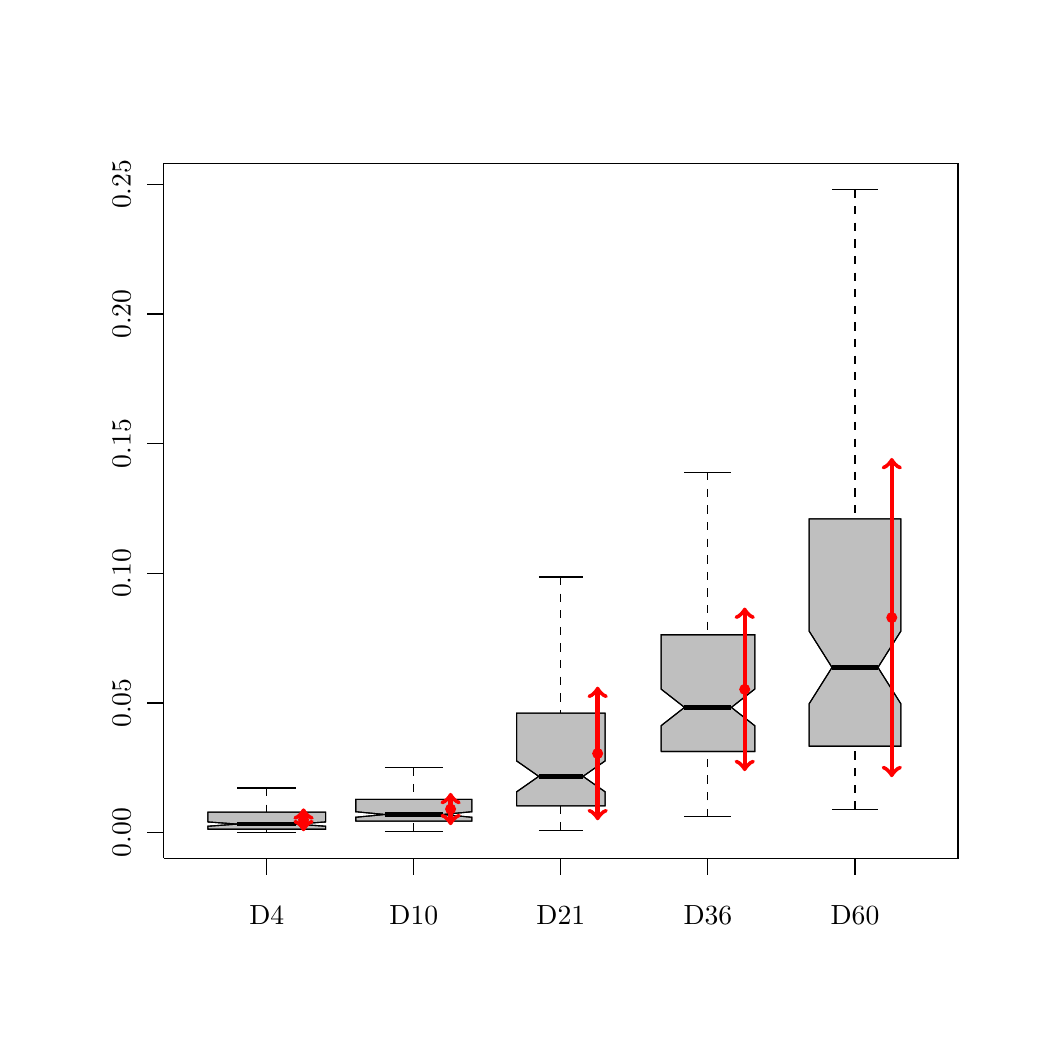
\begin{tikzpicture}[x=1pt,y=1pt]
\begin{scope}
\draw[fill=lightgray] ( 65.14, 71.70) --
	(107.65, 71.70) --
	(107.65, 72.79) --
	( 97.02, 73.56) --
	(107.65, 74.34) --
	(107.65, 77.88) --
	( 65.14, 77.88) --
	( 65.14, 74.34) --
	( 75.77, 73.56) --
	( 65.14, 72.79) --
	cycle;

\draw[ultra thick] ( 75.77, 73.56) -- ( 97.02, 73.56);

\draw[dashed] ( 86.40, 70.49) -- ( 86.40, 71.70);

\draw[dashed] ( 86.40, 86.59) -- ( 86.40, 77.88);

\draw[] ( 75.77, 70.49) -- ( 97.02, 70.49);

\draw[] ( 75.77, 86.59) -- ( 97.02, 86.59);

\draw[] ( 65.14, 71.70) --
	(107.65, 71.70) --
	(107.65, 72.79) --
	( 97.02, 73.56) --
	(107.65, 74.34) --
	(107.65, 77.88) --
	( 65.14, 77.88) --
	( 65.14, 74.34) --
	( 75.77, 73.56) --
	( 65.14, 72.79) --
	( 65.14, 71.70);

\draw[fill=lightgray] (118.55, 74.63) --
	(160.52, 74.63) --
	(160.52, 76.03) --
	(150.03, 77.03) --
	(160.52, 78.03) --
	(160.52, 82.51) --
	(118.55, 82.51) --
	(118.55, 78.03) --
	(129.04, 77.03) --
	(118.55, 76.03) --
	cycle;

\draw[ultra thick] (129.04, 77.03) -- (150.03, 77.03);

\draw[dashed] (139.54, 70.95) -- (139.54, 74.63);

\draw[dashed] (139.54, 94.09) -- (139.54, 82.51);

\draw[] (129.04, 70.95) -- (150.03, 70.95);

\draw[] (129.04, 94.09) -- (150.03, 94.09);

\draw[] (118.55, 74.63) --
	(160.52, 74.63) --
	(160.52, 76.03) --
	(150.03, 77.03) --
	(160.52, 78.03) --
	(160.52, 82.51) --
	(118.55, 82.51) --
	(118.55, 78.03) --
	(129.04, 77.03) --
	(118.55, 76.03) --
	(118.55, 74.63);

\draw[fill=lightgray] (176.68, 80.12) --
	(208.67, 80.12) --
	(208.67, 85.22) --
	(200.67, 90.81) --
	(208.67, 96.39) --
	(208.67,113.67) --
	(176.68,113.67) --
	(176.68, 96.39) --
	(184.68, 90.81) --
	(176.68, 85.22) --
	cycle;

\draw[ultra thick] (184.68, 90.81) -- (200.67, 90.81);

\draw[dashed] (192.67, 71.28) -- (192.67, 80.12);

\draw[dashed] (192.67,162.86) -- (192.67,113.67);

\draw[] (184.68, 71.28) -- (200.67, 71.28);

\draw[] (184.68,162.86) -- (200.67,162.86);

\draw[] (176.68, 80.12) --
	(208.67, 80.12) --
	(208.67, 85.22) --
	(200.67, 90.81) --
	(208.67, 96.39) --
	(208.67,113.67) --
	(176.68,113.67) --
	(176.68, 96.39) --
	(184.68, 90.81) --
	(176.68, 85.22) --
	(176.68, 80.12);

\draw[fill=lightgray] (228.87, 99.80) --
	(262.75, 99.80) --
	(262.75,109.10) --
	(254.28,115.73) --
	(262.75,122.36) --
	(262.75,141.97) --
	(228.87,141.97) --
	(228.87,122.36) --
	(237.34,115.73) --
	(228.87,109.10) --
	cycle;

\draw[ultra thick] (237.34,115.73) -- (254.28,115.73);

\draw[dashed] (245.81, 76.17) -- (245.81, 99.80);

\draw[dashed] (245.81,200.72) -- (245.81,141.97);

\draw[] (237.34, 76.17) -- (254.28, 76.17);

\draw[] (237.34,200.72) -- (254.28,200.72);

\draw[] (228.87, 99.80) --
	(262.75, 99.80) --
	(262.75,109.10) --
	(254.28,115.73) --
	(262.75,122.36) --
	(262.75,141.97) --
	(228.87,141.97) --
	(228.87,122.36) --
	(237.34,115.73) --
	(228.87,109.10) --
	(228.87, 99.80);

\draw[fill=lightgray] (282.35,101.68) --
	(315.55,101.68) --
	(315.55,116.98) --
	(307.25,130.16) --
	(315.55,143.34) --
	(315.55,183.85) --
	(282.35,183.85) --
	(282.35,143.34) --
	(290.65,130.16) --
	(282.35,116.98) --
	cycle;

\draw[ultra thick] (290.65,130.16) -- (307.25,130.16);

\draw[dashed] (298.95, 78.85) -- (298.95,101.68);

\draw[dashed] (298.95,302.86) -- (298.95,183.85);

\draw[] (290.65, 78.85) -- (307.25, 78.85);

\draw[] (290.65,302.86) -- (307.25,302.86);

\draw[] (282.35,101.68) --
	(315.55,101.68) --
	(315.55,116.98) --
	(307.25,130.16) --
	(315.55,143.34) --
	(315.55,183.85) --
	(282.35,183.85) --
	(282.35,143.34) --
	(290.65,130.16) --
	(282.35,116.98) --
	(282.35,101.68);
\end{scope}
\begin{scope}
\path[clip] (  0.00,  0.00) rectangle (361.35,361.35);
\definecolor[named]{drawColor}{rgb}{0.00,0.00,0.00}

\draw[] ( 86.40, 61.20) -- (298.95, 61.20);

\draw[] ( 86.40, 61.20) -- ( 86.40, 55.20);

\draw[] (139.54, 61.20) -- (139.54, 55.20);

\draw[] (192.67, 61.20) -- (192.67, 55.20);

\draw[] (245.81, 61.20) -- (245.81, 55.20);

\draw[] (298.95, 61.20) -- (298.95, 55.20);

\node[anchor=base,inner sep=0pt, outer sep=0pt] at ( 86.40, 37.20) {D4%
};

\node[anchor=base,inner sep=0pt, outer sep=0pt] at (139.54, 37.20) {D10%
};

\node[anchor=base,inner sep=0pt, outer sep=0pt] at (192.67, 37.20) {D21%
};

\node[anchor=base,inner sep=0pt, outer sep=0pt] at (245.81, 37.20) {D36%
};

\node[anchor=base,inner sep=0pt, outer sep=0pt] at (298.95, 37.20) {D60%
};

\draw[] ( 49.20, 70.47) -- ( 49.20,304.73);

\draw[] ( 49.20, 70.47) -- ( 43.20, 70.47);

\draw[] ( 49.20,117.32) -- ( 43.20,117.32);

\draw[] ( 49.20,164.18) -- ( 43.20,164.18);

\draw[] ( 49.20,211.03) -- ( 43.20,211.03);

\draw[] ( 49.20,257.88) -- ( 43.20,257.88);

\draw[] ( 49.20,304.73) -- ( 43.20,304.73);

\node[rotate= 90.00,anchor=base,inner sep=0pt, outer sep=0pt] at ( 37.20, 70.47) {0.00%
};

\node[rotate= 90.00,anchor=base,inner sep=0pt, outer sep=0pt] at ( 37.20,117.32) {0.05%
};

\node[rotate= 90.00,anchor=base,inner sep=0pt, outer sep=0pt] at ( 37.20,164.18) {0.10%
};

\node[rotate= 90.00,anchor=base,inner sep=0pt, outer sep=0pt] at ( 37.20,211.03) {0.15%
};

\node[rotate= 90.00,anchor=base,inner sep=0pt, outer sep=0pt] at ( 37.20,257.88) {0.20%
};

\node[rotate= 90.00,anchor=base,inner sep=0pt, outer sep=0pt] at ( 37.20,304.73) {0.25%
};
\end{scope}
\begin{scope}
\path[clip] (  0.00,  0.00) rectangle (361.35,361.35);
\draw ( 49.20, 61.20) --
	(336.15, 61.20) --
	(336.15,312.15) --
	( 49.20,312.15) --
	( 49.20, 61.20);
\end{scope}
\begin{scope}
\path[clip] ( 49.20, 61.20) rectangle (336.15,312.15);

\fill[color=red] ( 99.68, 75.11) circle (2);
\fill[color=red] (152.82, 79.00) circle (2);
\fill[color=red] (205.96, 99.07) circle (2);
\fill[color=red] (259.10,122.25) circle (2);
\fill[color=red] (312.24,148.19) circle (2);

\draw[<->,ultra thick,color=red] ( 99.68, 70.97) -- ( 99.68, 79.25);
\draw[<->,ultra thick,color=red] (152.82, 73.17) -- (152.82, 84.83);
\draw[<->,ultra thick,color=red] (205.96, 74.94) -- (205.96,123.21);
\draw[<->,ultra thick,color=red] (259.10, 92.70) -- (259.10,151.80);
\draw[<->,ultra thick,color=red] (312.24, 90.51) -- (312.24,205.86);

\end{scope}
\end{tikzpicture}
%-----------------------------------
%\end{document}
	\caption{BoxPlot of Data with removed outliers}
	\label{fig:boxplot}
\end{figure}

\begin{figure}
	\centering
	\pgfplotsset{width=.5\linewidth}
	\subfloat[Mean acinar volumes]{% !TEX root = ../acinus.tex

% \documentclass{article}
% \usepackage{tikz,pgfplots}
% \usepackage{siunitx}
% \usepackage[graphics,tightpage,active]{preview}
% \PreviewEnvironment{tikzpicture}
% \newcommand{\imsize}{\linewidth}
% \newlength\imagewidth           % needed for scalebars
% \newlength\imagescale           % ditto
% \begin{document}%
%%%%%%%%%%%%%%%%%%%%%%%%%%%%%%%%%%%%%%%%
	\begin{tikzpicture}
		\begin{axis}[%
			legend pos=south east,%
			scale only axis,%
			%ultra thick,%
			xlabel={Days},%
			ylabel={Volume [\si{\micro\litre}]},%
			xlabel near ticks,%
			ylabel near ticks,%
			xtick = data,%
			ytick = {0,0.02,...,0.11},%
			%ymajorgrids=true%
			]
			\addplot [blue,%
				mark=*,%
				semitransparent,%
				error bars/.cd,y dir=both,y explicit]
				coordinates {
 					(4,0.002595) +- (0.000308,0.000308)
					(10,0.012600) +- (0.001271,0.001271)
					(21,0.05602) +- (0.005973,0.005973)
					(36,0.084727) +- (0.006036,0.006036)
					(60,0.086460) +- (0.007447,0.007447)};
			\legend{Acini}
		\end{axis}
		\end{tikzpicture}
%%%%%%%%%%%%%%%%%%%%%%%%%%%%%%%%%%%%%%%%
% \end{document}
%Day	average	standard deviation	standard error of mean
%4	0.305	0.035	0.015
%10	0.508	0.048	0.022
%21	1.048	0.092	0.041
%36	2.062	0.141	0.063
%60	2.964	0.194	0.087}\\%
	\subfloat[Mean right lower lung lobe (RLL) volumes]{% !TEX root = ../acinus.tex

% \documentclass{article}
% \usepackage{tikz,pgfplots}
% \usepackage{siunitx}
% \usepackage[graphics,tightpage,active]{preview}
% \PreviewEnvironment{tikzpicture}
% \newcommand{\imsize}{\linewidth}
% \newlength\imagewidth           % needed for scalebars
% \newlength\imagescale           % ditto
% \begin{document}%
%%%%%%%%%%%%%%%%%%%%%%%%%%%%%%%%%%%%%%%%
	\begin{tikzpicture}
		%\tikzset{every mark/.append style={scale=4}}
		%\pgfplotsset{every axis legend/.append style={at={(0.8,0.08)},anchor=base}}
		\begin{axis}[%
			legend pos=south east,%
			scale only axis,%		
			%ultra thick,%
			xlabel={Days},%
			ylabel={Volume [\si{\centi\meter\cubed}]},%
			xlabel near ticks,%
			ylabel near ticks,%
			xtick = data,%
			%ytick = {0,5,...,35},%
			%ymajorgrids=true%
			]
			\addplot [red,%
				mark=square*,%
				semitransparent,%
				error bars/.cd,y dir=both,y explicit]
				coordinates {
 					(4,0.305) +- (0.015,0.015)
					(10,0.508) +- (0.022,0.022)
					(21,1.048) +- (0.041,0.041)
					(36,2.062) +- (0.063,0.063)
					(60,2.964) +- (0.087,0.087)};
		\legend{RLL}
		\end{axis}
		\end{tikzpicture}
%%%%%%%%%%%%%%%%%%%%%%%%%%%%%%%%%%%%%%%%
% \end{document}
%Day	average	standard deviation	standard error of mean
%4	0.305	0.035	0.015
%10	0.508	0.048	0.022
%21	1.048	0.092	0.041
%36	2.062	0.141	0.063
%60	2.964	0.194	0.087}\\%
	\subfloat[Volume increase based on day 4]{% !TEX root = ../acinus.tex

% \documentclass{article}
% \usepackage{tikz,pgfplots}
% \usepackage{siunitx}
% \usepackage[graphics,tightpage,active]{preview}
% \PreviewEnvironment{tikzpicture}
% \newcommand{\imsize}{\linewidth}
% \newlength\imagewidth           % needed for scalebars
% \newlength\imagescale           % ditto
% \begin{document}%
%%%%%%%%%%%%%%%%%%%%%%%%%%%%%%%%%%%%%%%%
	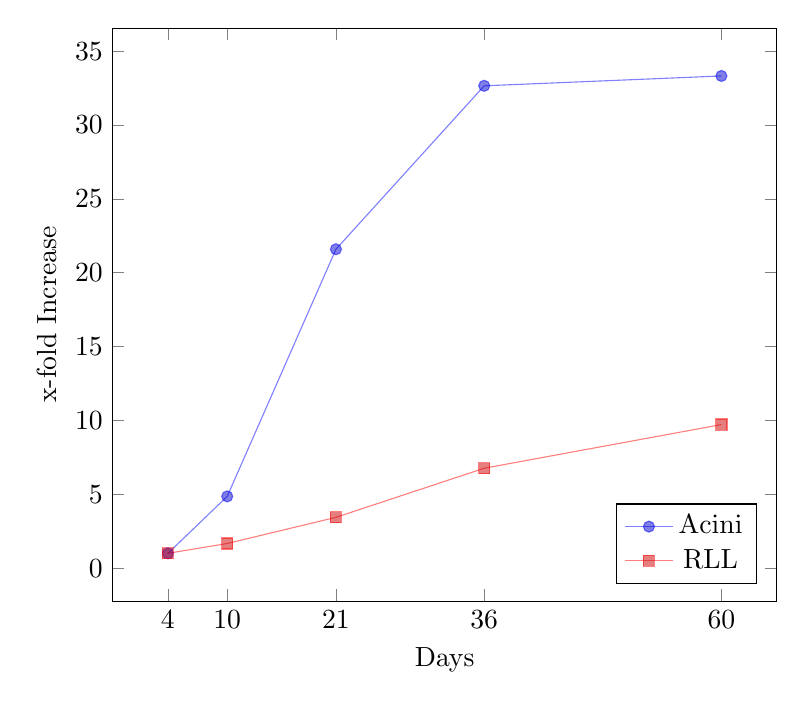
\begin{tikzpicture}
		\begin{axis}[%
			legend pos=south east,%
			scale only axis,%		
			%ultra thick,%
			xlabel={Days},%
			ylabel={x-fold Increase},%
			xlabel near ticks,%
			ylabel near ticks,%
			xtick = data,%
			ytick = {0,5,...,35},%
			%ymajorgrids=true%
			]
		\addplot+[semitransparent]
			coordinates{
		 		(4,1)
				(10,4.85549)
				(21,21.58767)
				(36,32.65010)
				(60,33.31792)
		};
		\label{plot:acini}
		\addplot+[semitransparent]
			coordinates{
				(4,1)
				(10,1.666)
				(21,3.436)
				(36,6.761)
				(60,9.718)
		};
		\label{plot:rul}
		\legend{Acini,RLL}
		\end{axis}
		\end{tikzpicture}
%%%%%%%%%%%%%%%%%%%%%%%%%%%%%%%%%%%%%%%%
% \end{document}}%
	\caption{Plot of increase in Volume for both Acini (\ref{plot:acini}) and right lower lung lobe (RLL, \ref{plot:rul}). While the volume of the right lower lung lobe increases approximately 10-fold over the first 2 months after birth, we see an approximately 33-fold increase in mean volume for the extracted acini from day \numrange{4}{60}.}
	\label{plot}
\end{figure}

We observed an approximately thirty-three-fold increase of the mean acinar volume during the postnatal lung development from days \numrange{4}{60} (33.25-fold, from \SIrange{0.00260}{0.08646}{\micro\litre}). During the same period the volume of the right lower lung lobe increases only approximately ten-fold (9.72-fold, from \SIrange{0.305}{2.964}{\centi\metre\cubed}, see \cite{Tschanz2003}), which results in an acinar growth 3.4 times larger than the right lower lung lobe volume.

\section{Discussion}\label{sec:Discussion}
We hypothesize that this large increase of the acinar volume can only be achieved by a conversion of the \numrange{2}{4} most distal purely conducting airways into alveolar ducts between birth and adulthood. As a consequence \numrange{4}{16} small acini have to be merged to a larger one. We expect that the increased complexity of the adult acini influences both ventilation and particle deposition.

\section{Acknowledgments}
We thank Federica Marone, Beamline Scientist at TOMCAT for the long-standing great support at the Beamline and implementation of the reconstruction of the merged wide-field scanning projections on the TOMCAT cluster. Christoph Hinterm\"{u}ller, former member of the TOMCAT group, and now Project Management \& Research at \href{http://gtec.at/}{g.tec medical engineering GmbH} also helped us during countless shifts at the beamline. He also helped with the first implementation of wide-field scanning at TOMCAT. Bernd Pinzer, Post Doc at TOMCAT adopted the support of our group from Chris and also does great job. Milo Hindennach, MeVis Developer at Fraunhofer MEVIS provided the \href{http://www.mevis-research.de/cgi-bin/discus/board-auth.cgi?lm=1282233250&file=/839/11760.html}{first ideas of a Manhole cover module in MeVisLab}, which is still at the core of the MeVisLab-network used in this publication. Sébastien Barré, Ph.\,D.\,Student in our group\todo{Or is he also on the author list?} was helping with preparations of the samples, data acquisition and preprocessing of the datasets. We thank Mohammed Ouanella, our former lab technician, for expert technical assistance in the lab. This work has been funded by the grants 3100A0-109874 and 310030-125397 \todo{Still correct?} of the Swiss National Science Foundation.

\bibliographystyle{unsrtnat}
\bibliography{../references}
 
\end{document}